\subsection{Expérience}
\label{subsec:experience}

L'expérience embarquée à bord de la fusée SP-02, comme énoncé précédemment, repose en très grande partie sur le projet antérieur
\gls{APEX}. Une amélioration du système sera effectué notamment au niveau de l'ajout d'un port externe où sera brancher un tube
pitot, permettant de mesurer la vitesse dynamique durant le vol, et à l'ajout d'un deuxième module de télémesure. L'idée est que
le module de télémesure déjà présent sur la carte \gls{APEX} sert à transmettre les données d'état de vol et de position
\acrshort{GNSS} via une modulation \acrshort{LORA} avec une faible vitesse de transmission mais une grande portée et un
\acrshort{SNR} importante. Le second module de télémesure, dédié à l'expérience, transmettra les données issues des capteurs.
Ce module utilisera une modulation \acrshort{FSK} à plus haute vitesse de transmission mais avec une portée plus faible.\\

Comme chaque étage est composé de sa propre carte \gls{APEX}, la fusée SP-02 embarquera donc 4 modules de télémesure, deux par
étage. Comme 2 modulations sont utilisées, le projet nécessitera 2 fréquences différentes dédiées. La différentiation de deux
module utilisant la même modulation sera assurée par l'utilisation de deux channels temporelles différents.\\

\begin{figure}[h!]
    \centering
    \begin{subfigure}{\textwidth}
        \centering
        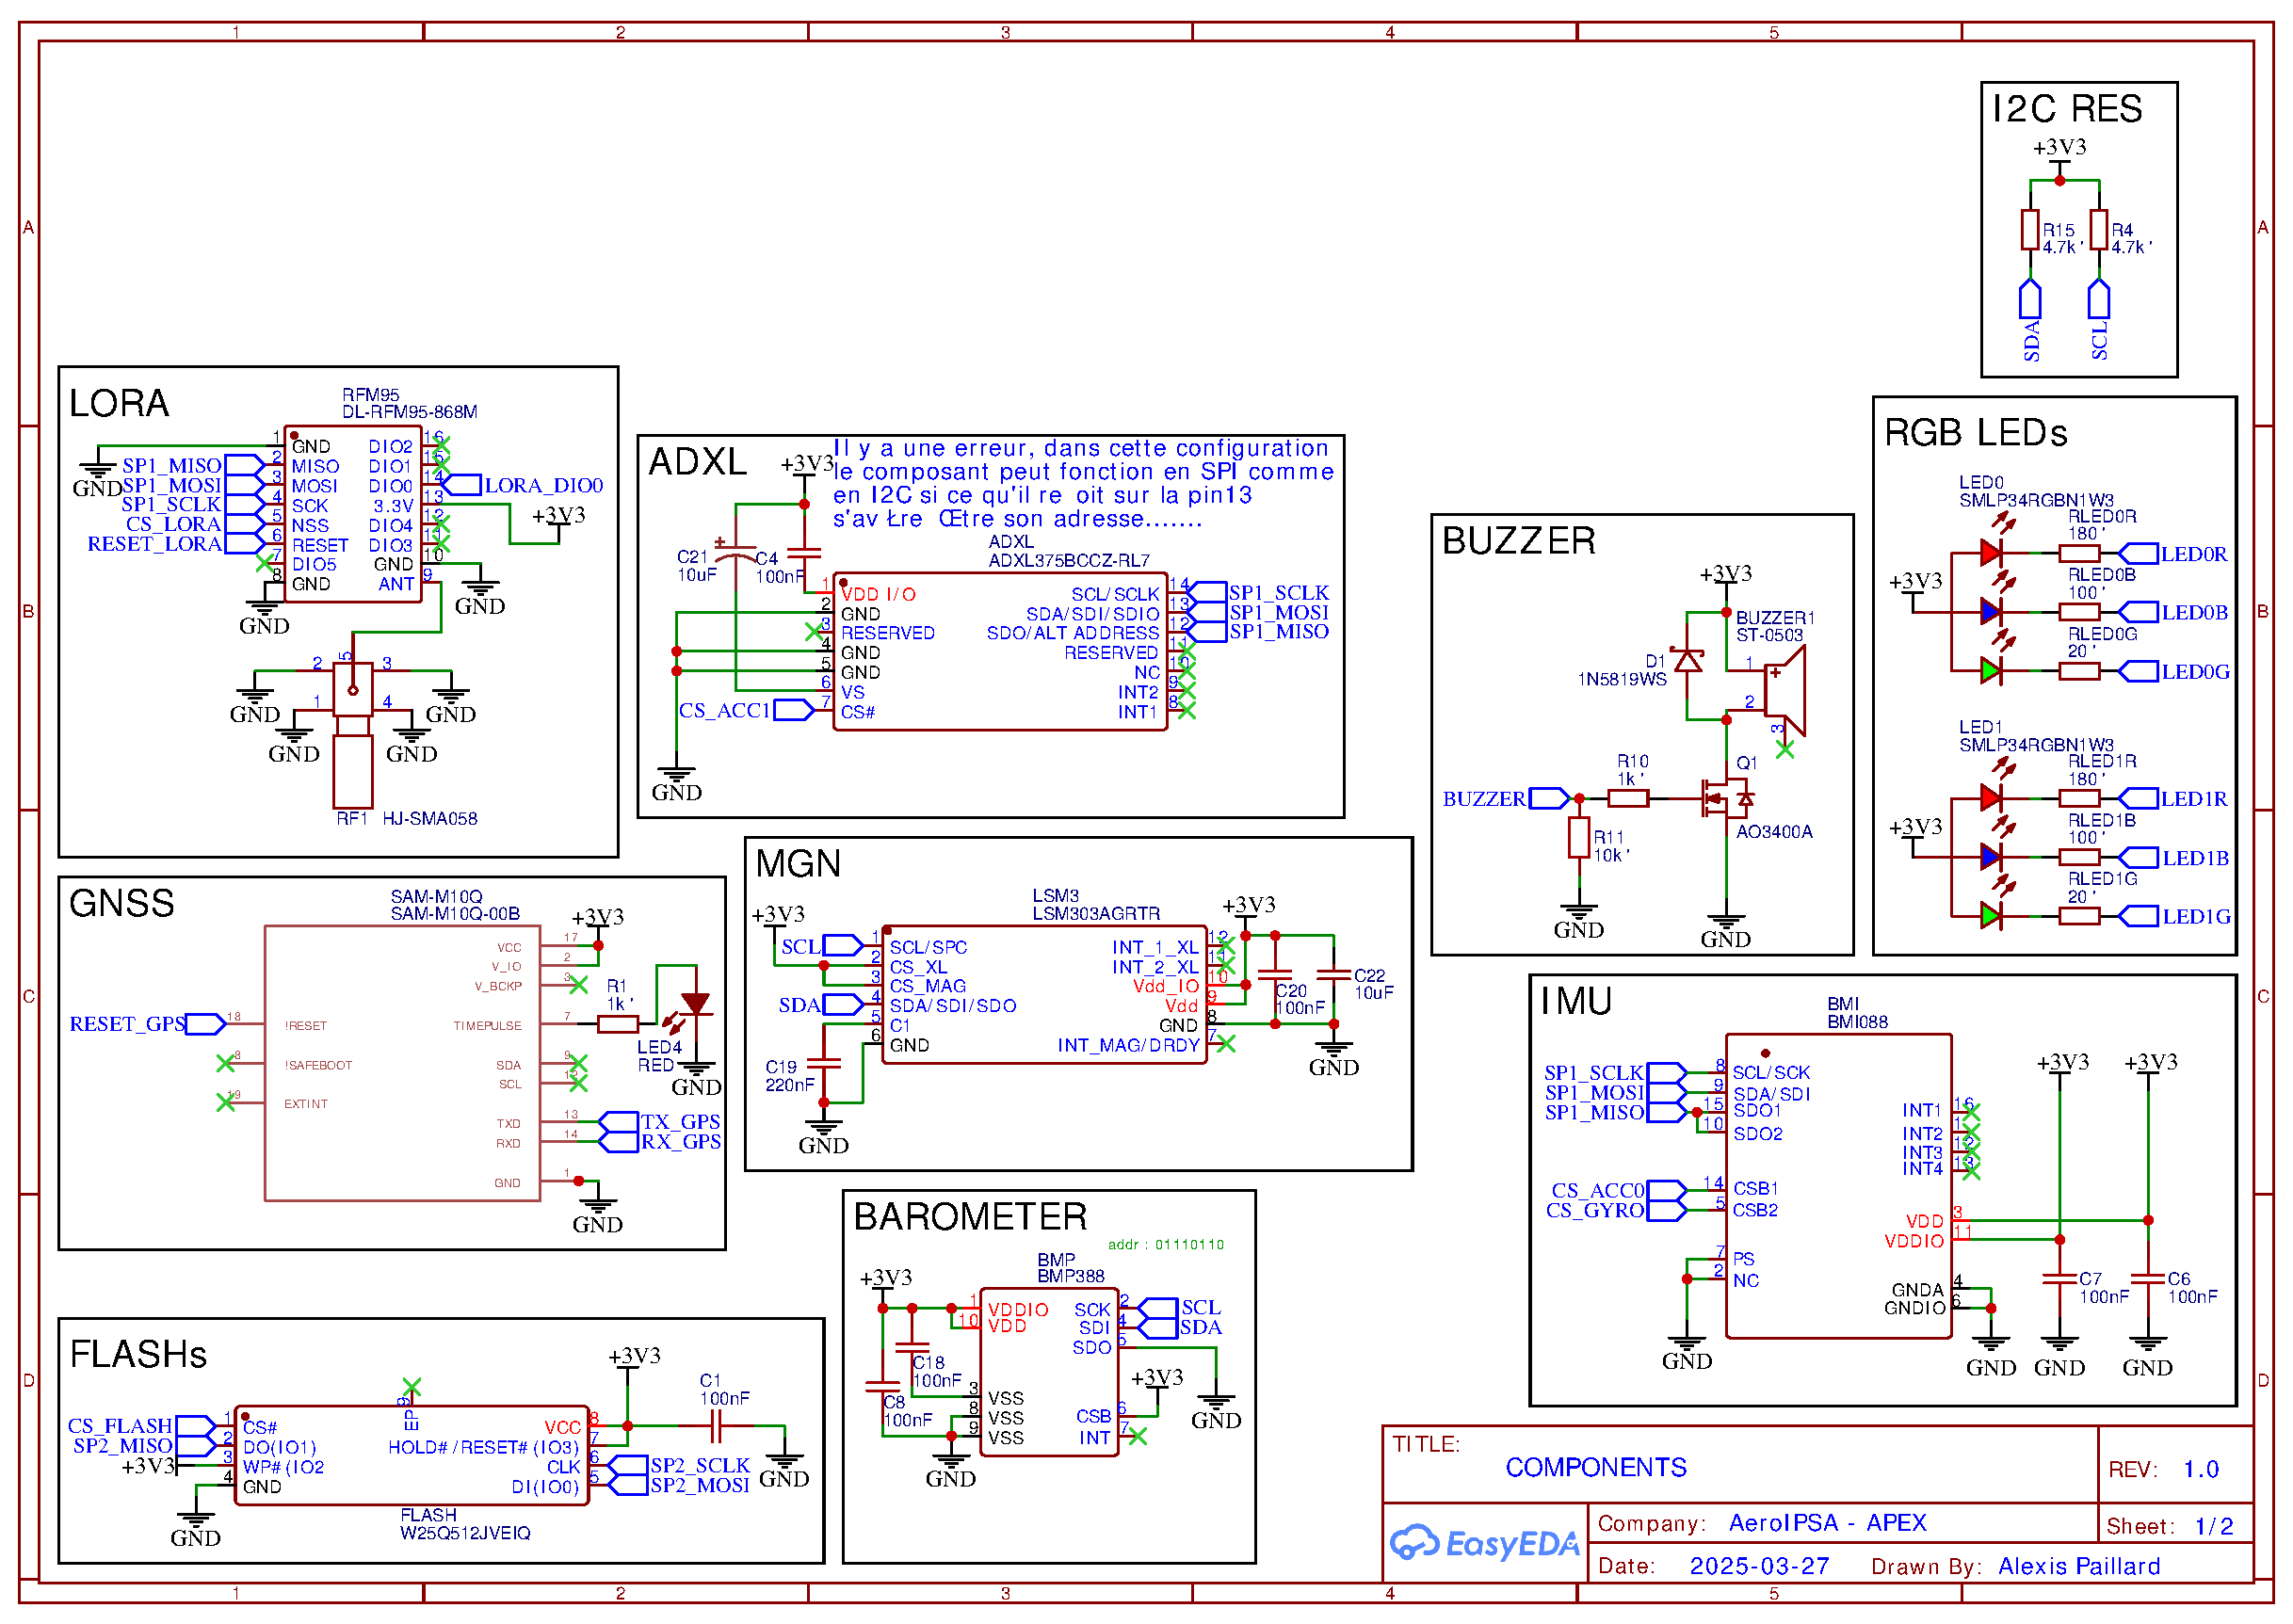
\includegraphics[width=0.6\textwidth]{figures/Sheet_1.pdf}
        \caption{Schéma 1}        
    \end{subfigure}
    \begin{subfigure}{\textwidth}
        \centering
        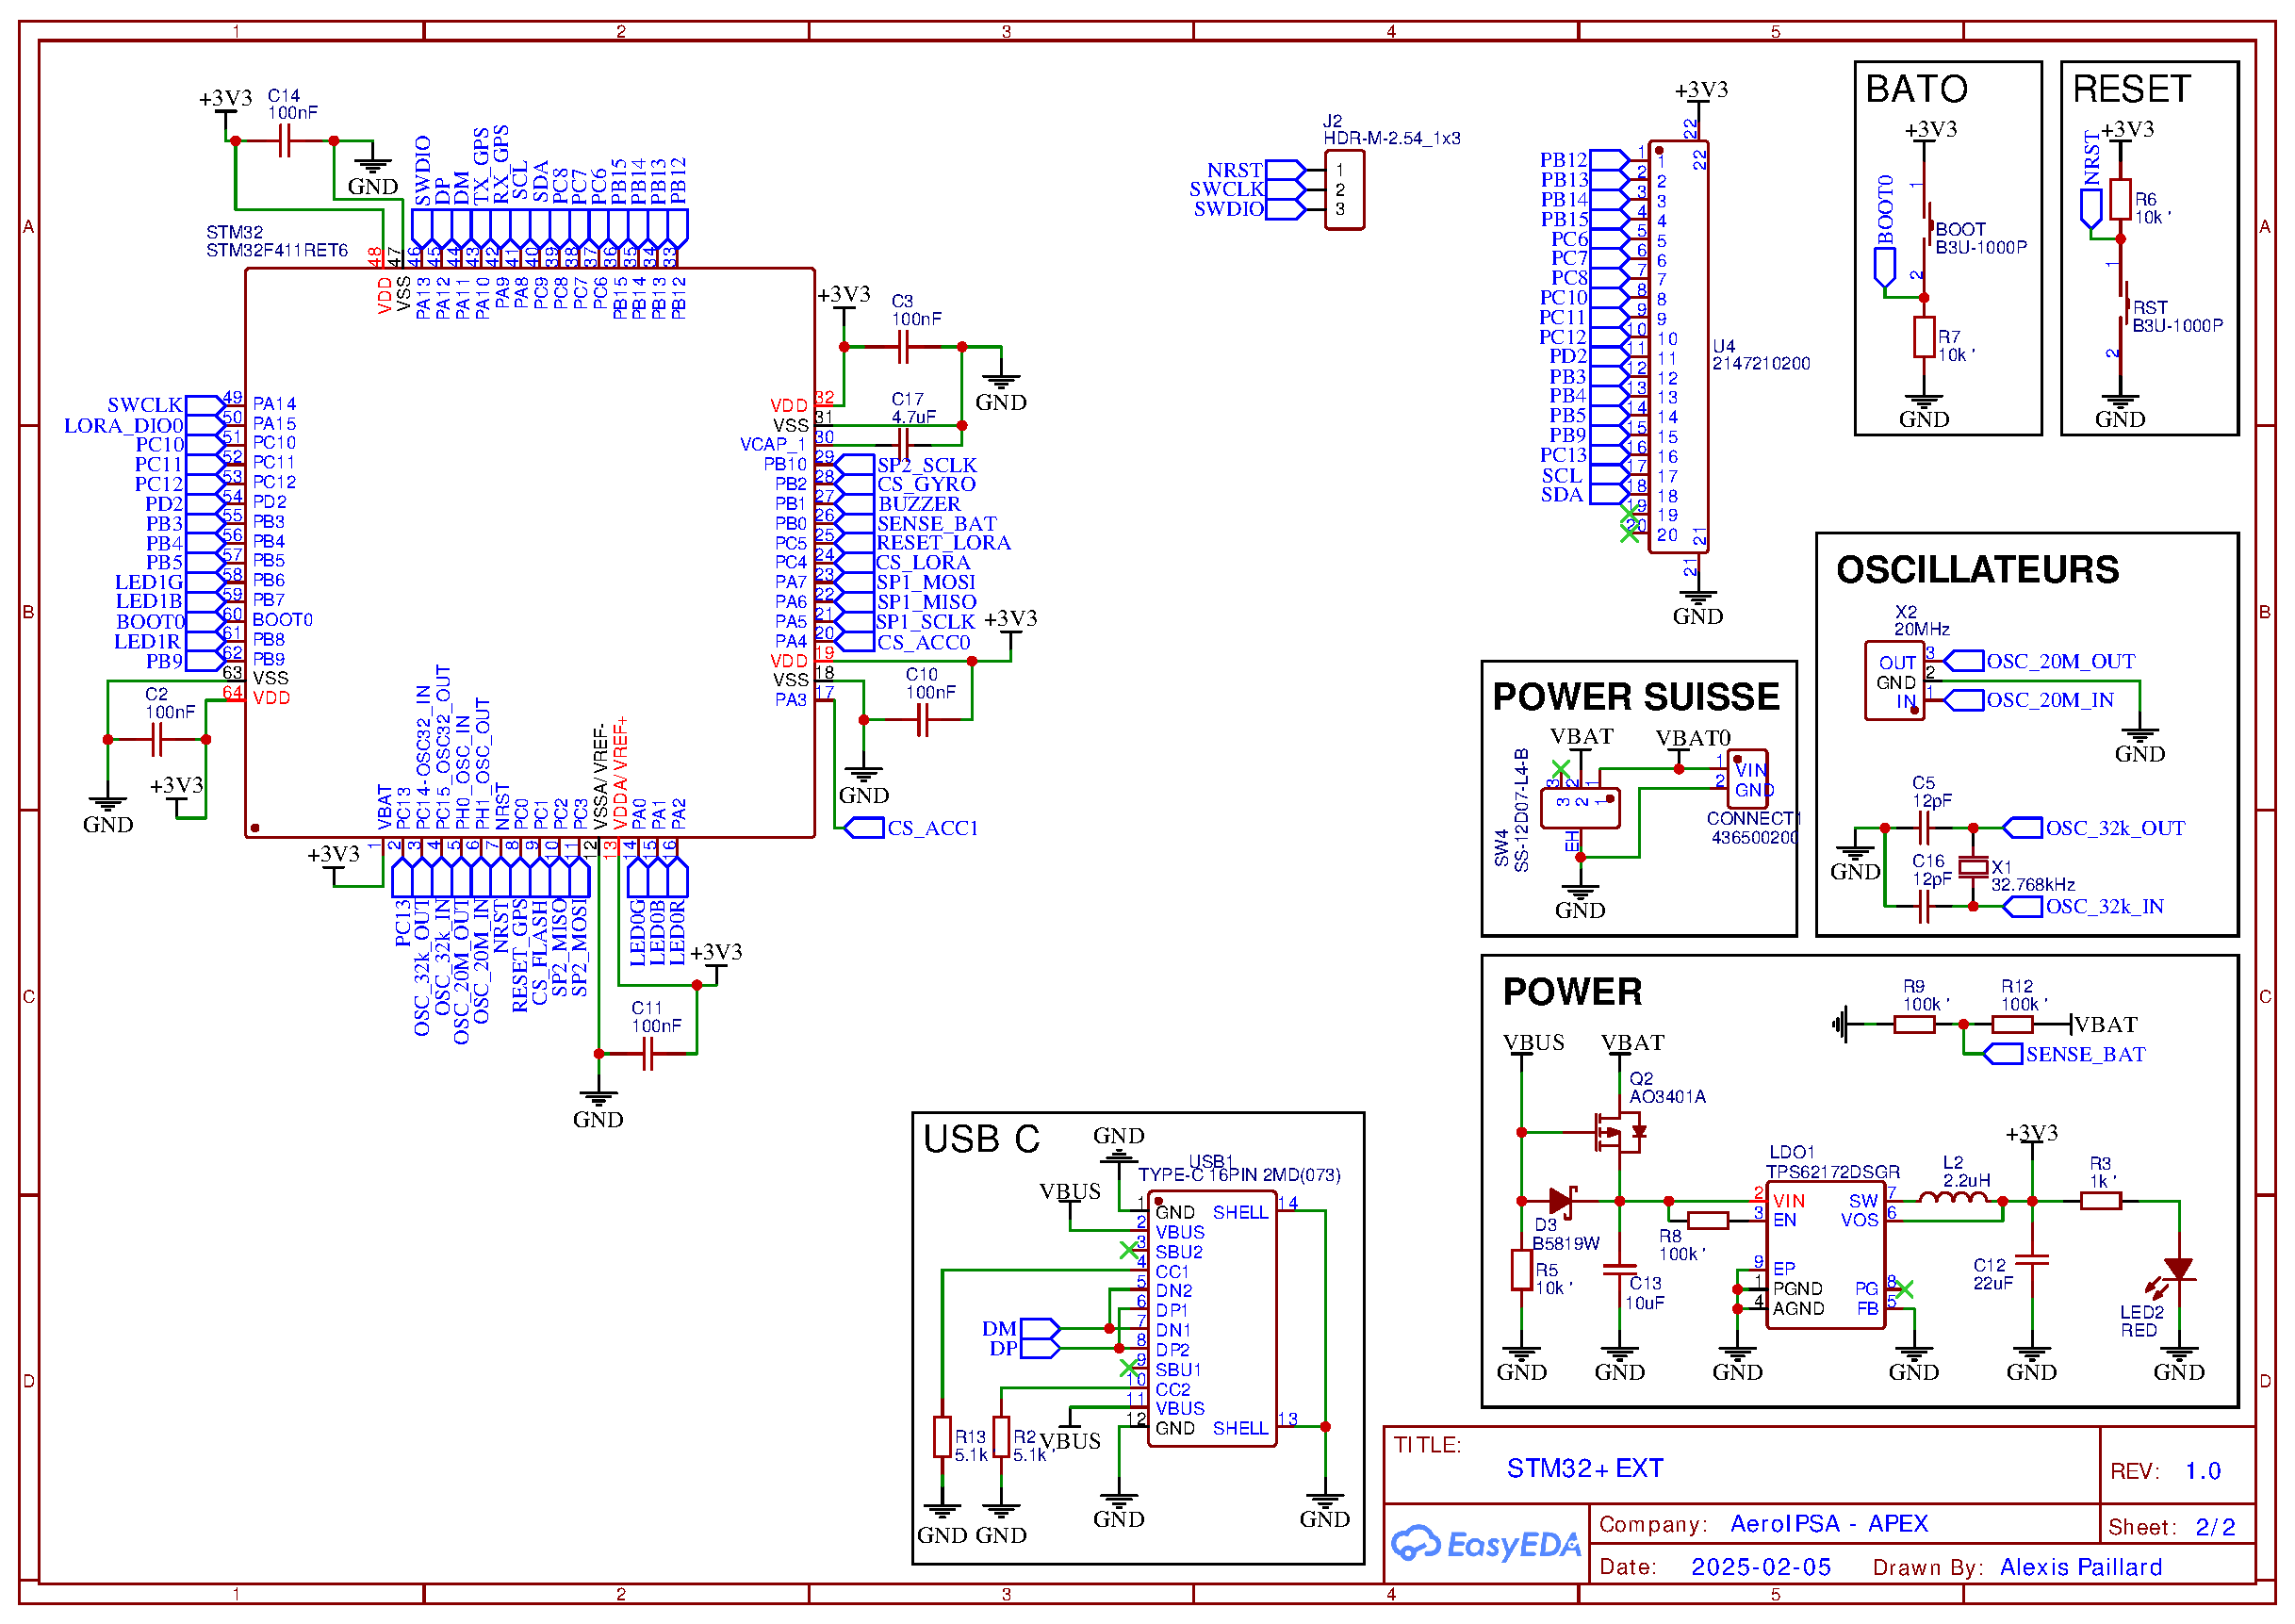
\includegraphics[width=0.6\textwidth]{figures/Sheet_2.pdf}
        \caption{Schéma 2}
    \end{subfigure}
    \caption{Schémas électriques de la carte APEX améliorée pour SP-02}
    \label{fig:schema_apex_sp02}
\end{figure}
